%\documentclass[a4j,twocolumn,uplatex]{jsarticle}
\documentclass[a4j,twocolumn,uplatex]{jarticle}
\usepackage[dvipdfmx]{graphicx}
\usepackage{wrapfig}	
\usepackage[dvipdfmx]{graphicx}
\usepackage{url}
\usepackage{here}
\usepackage{subfigure}
\usepackage[dvipdfmx]{graphics}
\usepackage{comment}
\usepackage{subfigure}
\setlength{\textheight}{275mm}
\headheight 5mm
\topmargin -30mm
\textwidth 185mm
\oddsidemargin -15mm
\evensidemargin -15mm
\pagestyle{empty}
\def\Vec#1{\mbox{\boldmath $#1$}}
\usepackage[dvipdfmx]{graphics}
\usepackage{comment}
\usepackage{subfigure}



\begin{document}
\title{Processing言語によるホイヘンスの原理の視覚化}
\author{情報科学科 西谷研究室3518 村上 大貴}
\date{}
\maketitle
\section{目的}
\vspace{-0.5em}
現在,政府は2020年を目標に中学および高等学校の全生徒がタブレットを携行するという計画を立てている\cite{tablet}.
タブレット端末を学習に利用する利点として,インタラクティブな教材を使用できる点があるが,このような教材が効力を発揮する教科の一つに物理がある.
例えば高校物理で学習するホイヘンスの原理は,実世界には存在しない素元波という概念を用いて波面を決定していく. これによって回折現象や,反射・屈折といった性質を矛盾なく説明できる反面,実世界にないが故に直観的な理解を得るのは難しい.
これを直観的に理解させ,学習を促進する手段として,物理現象の視覚化が適していると考えた.

本研究ではホイヘンスの原理を用いて波の回折現象や反射,屈折の性質を視覚化する学習支援プログラムの作成を目的とする.
%(タブレット上で動作することはいれるべきか?まだやしやめとこ)
インターラクティブな操作性や,タブレット上での動作に,アニメーションに優れた開発環境を提供するProcessing言語を用いる. 

\vspace{-2em}
\section{手法}
\vspace{-0.5em}
Processing言語はつぎのような特徴を有している\cite{ishikawa},
\begin{enumerate}
\item インタラクティブソフトウェアやビジュアルプレゼンテーションを用意に実現することに特化している.
\item Windows, iOS, Androidのタブレット端末で用いられる3つのプラットフォーム全てで動作する. 
\end{enumerate}
これらの理由から,本研究のプログラムの開発言語として最も適していると考え,採用した.

\vspace{-1em}
\paragraph{素元波の考え方}
ホイヘンスの原理を教科書は以下のように記している.「1つの波面上の全ての点は,それらを波源とする球面波(素元波)を発生させ,素元波の共通に接する面が次の瞬間の波面となる.これをホイヘンスの原理という」\cite[p.195]{kyoukasyo}.つまり,素元波は一つ一つは見えないものの,その性質は普通の波とかわらずその重ね合わせとなる.今回作成するプログラムでは,波源とそこからの素元波を波長,周期,振幅といった要素をもたせて描写処理を行っている.


\vspace{-2em}
\section{開発結果}
\vspace{-0.5em}
\paragraph{波の干渉}
回折,反射,屈折の性質を可視化するには,多数の波が干渉する様子を忠実に再現しなければならないため,図\ref{fig:program1}(a)の波の干渉を視覚化するプログラムを作成した. ユーザは,描写領域上の任意の座標に波源を設定でき,波源ごとに生成されるスライダーによって波の周期と波長を変更することができる.
また,変位の数値を確認できれば理解の促進につながると考え,図\ref{fig:program1}(b)の,指定したy座標での波の変位を動的にグラフにプロットする機能も作成した.

\begin{figure}[H]
\subfigure[2次元での高低のカラー表示.]
{\mbox{\raisebox{1mm}
{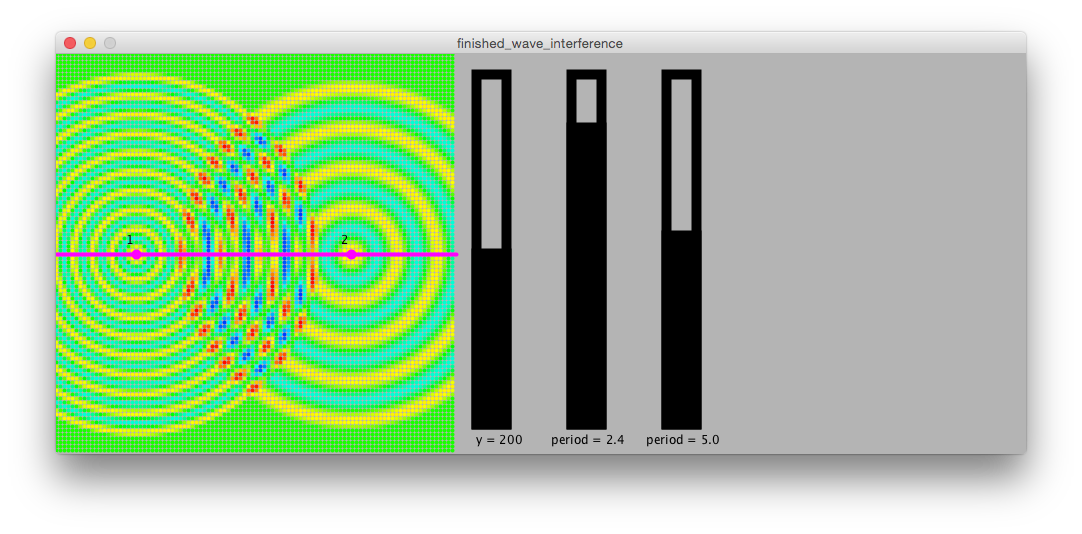
\includegraphics[keepaspectratio, scale = 0.115]
{./interference.png}}}}
\subfigure[横軸断面での変位.]
{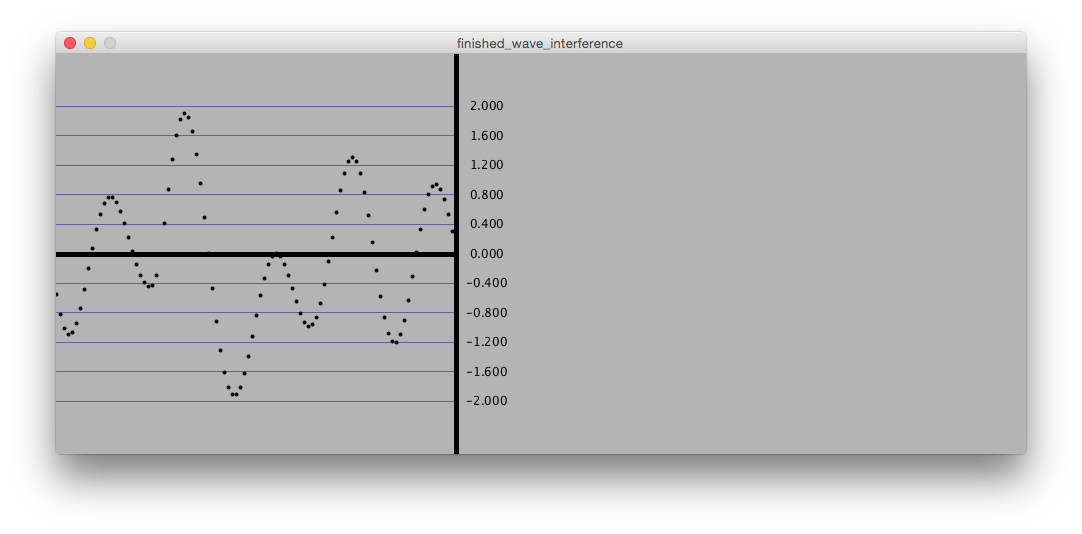
\includegraphics[keepaspectratio, scale = 0.115]
{./check.png}}
\caption{{\footnotesize 干渉波のプログラム表示.}}
\label{fig:program1}
\end{figure}
%\vspace{-7mm}

\vspace{-5mm}
\paragraph{スリット回折}
波の干渉の視覚化プログラムでの処理をベースとして,図\ref{fig:program2}のスリット回折現象を視覚化するプログラムを作成した.画面右のスライダーによって素元波の波長を変更することにより,図\ref{fig:program2}(a)から(b)のように回折の度合いが変わる.またスリット間隙もプログラム起動時に調整でき,これによって,「回折現象はスリット間隙と波長の長さの相対的な度合いに左右される」ということがわかりやすくなった.
%プレゼンでは障害物の隙間の間隔も回折に関係してくることを示す.
\begin{figure}[H]
\subfigure[波の干渉.]
{\mbox{\raisebox{1mm}
{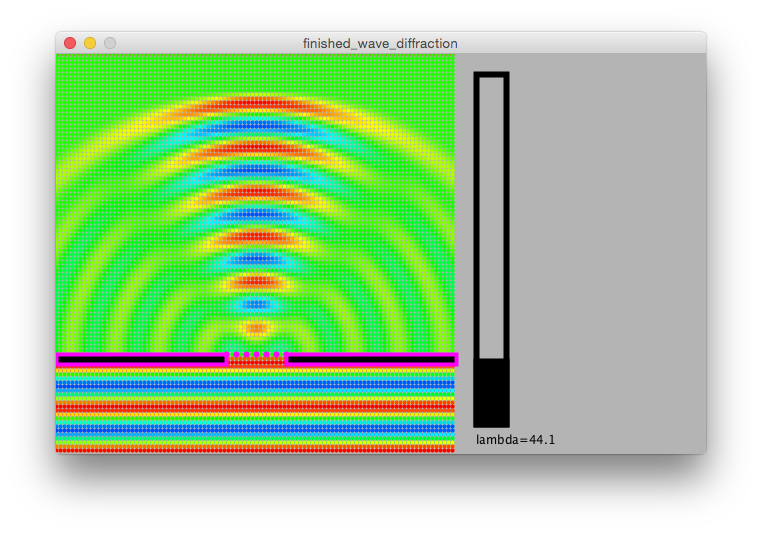
\includegraphics[keepaspectratio, scale = 0.16]
{./diffraction1.png}}}}
\subfigure[波の回折が大きい場合.]
{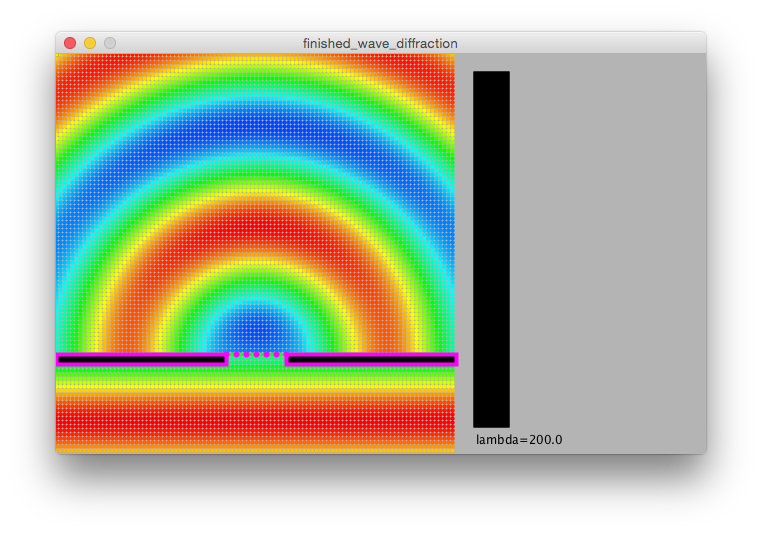
\includegraphics[keepaspectratio, scale = 0.16]
{./diffraction2.png}}
%\caption{{\footnotesize 波の性質と素元波\cite{kyoukasyo}.}}
\caption{{\footnotesize 波の回折現象を視覚化したプログラム.}}
\label{fig:program2}
\end{figure}

\vspace{-2em}
\section{今後の課題}
\vspace{-0.5em}
反射角,屈折角の描写では理論とすこし隔たりがあるため,その精度を向上させる必要がある.また教育現場で利用できる完成したプログラムとするには,操作性などのデザイン性を向上させる必要がある.
\vspace{-5mm}
\begin{thebibliography}{9}
\bibitem{tablet} 文部科学省,\url{http://www.mext.go.jp/b_menu/houdou/23/04/__icsFiles/afieldfile/2011/04/28/1305484_01_1.pdf}, p34.
\bibitem{ishikawa} 石川将人,北卓人,大須賀公一, 自動制御連合講演会講演論文集, {\bf 53}(0), (2010), p.247.
\bibitem{kyoukasyo} 「物理I」, 中村 英二ほか,(学習社 2004).
\end{thebibliography}
\end{document}


